% Preamble --------------------------------------------------------

\documentclass[a4paper]{article}
\usepackage[utf8]{inputenc}

\usepackage{lipsum}     % space filling
\usepackage{xspace}     % for commands
\usepackage[colorlinks=true, allcolors=blue]{hyperref} % to control how hyperlinks look
\usepackage[version=4]{mhchem} % chemistry
\usepackage{microtype}  % better justified paragraphs
\usepackage{graphicx}   % better control of figures
\usepackage{booktabs}   % toprule/bottomrule/midrule
\usepackage{tabularx}   % tabularx environ
\usepackage{amsmath}    %useful package for mathematical notation

\usepackage[backend=biber,
natbib=true,
style=authoryear,
sorting=none,
maxbibnames=99,
backref=true, % show page numbers where reference used
url=true
]{biblatex}

\addbibresource{bib/refs.bib}

% different fonts, see https://tug.org/FontCatalogue/ for options
%\usepackage{tgpagella}
\usepackage{XCharter}
%\usepackage[sfdefault]{noto}
\usepackage[T1]{fontenc}

\title{My \LaTeX~Document}
\author{Jack~Davison\thanks{Wolfson Atmospheric Chemistry Laboratories} \and Shona~E.~Wilde\footnotemark[1] \and Craig~Poku\footnotemark[1] \and David~C.~Carslaw\footnotemark[1]\thanks{Ricardo Energy \& Environment}}
\date{December 2021}

% examples of macros to help make things easier to type
\newcommand{\nox}{\ce{NO_x}\xspace}
\newcommand{\pmtwo}{\ce{PM_{2.5}}\xspace}
\newcommand{\cotwo}{\ce{CO_2}\xspace}
\newcommand{\nhthree}{\ce{NH_3}\xspace}
\newcommand{\ug}{\textmu g~m$^{-3}$\xspace}




% Document --------------------------------------------------------

\begin{document}

\maketitle

\tableofcontents

\newpage

\section{Introduction}

Your introduction goes here! Simply start writing your document and use the Recompile button to view the updated PDF preview. Examples of commonly used commands and features are listed below, to help you get started.

With shortcut macros it is easy to write chemical names / units etc., such as \nox and \pmtwo and \nhthree \ldots all in \ug.

We can even really easily format chemical names, like this long (and fictional!) species: \ce{C2H3O8N2S^2+}.

\subsection{How to add Lists}

You can make lists with automatic numbering \dots

\begin{enumerate}
\item Like this,
\item and like this.
\end{enumerate}
\dots or bullet points \dots
\begin{itemize}
\item Like this,
\item and like this.
\end{itemize}

\section{Methods}

\subsection{Sections and Subsections}

You can have sections, subsections and \textit{sub}subsections to split up your document. All can be labelled and later referred to. For example, we'll be talking about maths in \autoref{ssec:math} and tables in \autoref{ssec:table}. If we added additional subsections before these, \LaTeX would automatically update their numbers. 

\subsection{Maths}\label{ssec:math}

LaTeX is super useful when it comes to writing equations. So if I want to change anything into mathematical text, I can surround text with \$ signs, which will turn y = mx + c into $y = mx + c$. I can also use LaTeX to make equations into their own separate lines,

$A+B = C$

and therefore turning $y = mx + c$ into \autoref{eq:linear};

\begin{equation}\label{eq:linear}
    y = mx + c.
\end{equation}

Having the flexibility to define equations both outside and inline with the text makes writing maths in LaTeX pretty useful when working on long documents. For example, suppose we want to know the answer for a super complicated equation:

\begin{align}\label{eq:integral}
    \int^{\infty}_{-\infty} e^{-x^2} dx  &= X  \\
        Y  &= X
\end{align}

We can define our answer for \autoref{eq:integral} either as $X = \sqrt{\pi}$, or in its own equation line as:

\begin{equation}
    X = \sqrt{\pi},
\end{equation}

which you may decide to change depending on your specific needs. Finally, a useful tool to have if you're doing something maths heavy is the \texttt{amsmath} package. See this incredibly long equation, \autoref{eq:long}.

\begin{equation}\label{eq:long}
    F = \{F_{x} \in  F_{c} : (|S| > |C|) \cap 
(\tau  < |S| < \beta) \cap 
(|S_{i}| > |S| - \epsilon)
  \},
\end{equation}

Some journals want you to have have the full word "Equation" and instead want "Eq.". Using \texttt{amsmath}, you can use the function \texttt{eqref}, allowing you refer to our super long equation as either \autoref{eq:long} or Eq. \eqref{eq:long}.

\section{Discussion} \label{sec:disc}

\subsection{Tables} \label{ssec:table}

Tables live inside of ``tabular'' environments which you'd usually contain inside of ``table'' environments. The syntax can be slightly strange, but gives you a high amount of control over table layouts. There are useful packages to enhance the use of tables - ``booktabs'' enhances their appearance, ``tabularx'' can \textit{justify} tables, and ``longtable'' allows for tables to be split across multiple pages.

An example of a table is found in \autoref{tab:nox_table}, using ``booktabs'' to add horizontal lines.

\begin{table}[bht]
    \centering
    \begin{tabular}{l l l l}
    \toprule
                        &               & \multicolumn{2}{l}{\textbf{Emissions}} \\ \cmidrule(r){3-4}
         \textbf{Fuel}  & \textbf{Type} & \textbf{\nox} & \textbf{CO} \\
    \midrule
         Diesel & Cars & High & Low \\
         Petrol & Cars & Low & High \\
         Diesel & Heavy & Really high! & Low  \\
    \bottomrule
    \end{tabular}
    \caption{\nox and CO emissions from different vehicle types.}
    \label{tab:nox_table}
\end{table}

A wider table is shown in \autoref{tab:wide_tab}, justified to be the width of the text using the ``tabularx'' package.

\begin{table}[bht]
    \centering
    \begin{tabularx}{\linewidth}{lXXXX}
        \toprule
        \textbf{Species} & \textbf{Petal Length} & \textbf{Petal Width} & \textbf{Sepal Length} & \textbf{Sepal Width} \\ 
        \midrule
        Setosa & 1.462 & 0.246 & 5.006 & 3.428 \\ 
        Versicolor & 4.260 & 1.326 & 5.936 & 2.770 \\ 
        Virginica & 5.552 & 2.026 & 6.588 & 2.974 \\ 
        \bottomrule
    \end{tabularx}
    \caption{Mean values from Fischer's ``iris'' data set.}
    \label{tab:wide_tab}
\end{table}

\subsection{Figures}

Figures can be inserted in a ``figure'' environment. The important things to include are:

\begin{enumerate}
    \item ``includegraphics'', which needs a path to your image. This also allows you to define the width of the figure if you have the ``graphicx'' package loaded.
    \item A ``caption'' to describe your figure. 
    \item A ``label'' so you can refer to your figure in-text
    \item The ``centering'' command, so that the figure is centred on the page.
\end{enumerate}

It's a good idea for your figures to be \textbf{vectors} rather than \textbf{rasters}. This means that they won't look really blurry when zoomed in! It'll also make them more scalable if you want to put them on slides or an A0 conference poster. An example of a PDF figure is found in \autoref{fig:mtcars}.

\begin{figure}[bht]
    \centering
    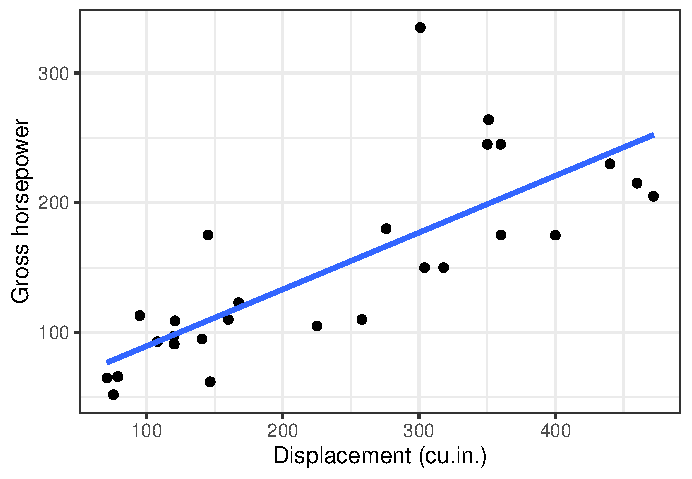
\includegraphics[width=.8\linewidth]{plots/myplot.pdf}
    \caption{A lovely R plot, saved as a PDF rather than a PNG or JPEG.}
    \label{fig:mtcars}
\end{figure}

\subsection{References}

Some examples of recent papers \citep{Davison2020, Wagner2021ApplicationGases, Farren2020UnderestimatedVehicles, Farren2021CharacterisationCars}. Or we can talk about them in-text; \citet{Carslaw2011} is an example. 

\newpage

{\sloppy\printbibliography}

\end{document}
